% 原 PPT 第 4 页；共 3 个显示状态。
\begin{frame}<1-3>[t]{\fitcampustitle{求函数的解析式}}
\begin{campuscanvas}
\only<1|handout:0>{\node[anchor=north west,inner sep=0] at (25.600,116) {\includegraphics[page=7,width=153.6000mm]{source-content/content.pdf}};}
\only<2|handout:0>{\node[anchor=north west,inner sep=0] at (25.600,116) {\includegraphics[page=8,width=153.6000mm]{source-content/content.pdf}};}
\only<3|handout:1>{\node[anchor=north west,inner sep=0] at (25.600,116) {\includegraphics[page=9,width=153.6000mm]{source-content/content.pdf}};}
\end{campuscanvas}
\end{frame}
